\section{The Analysis}
\label{sec:Analysis}
In this work we analyse the data from \Xehund\ `s scientfic run II ~\cite{xe100_run10_si,xe100_run10_sd} , taken between February 28th,2011 and March 31st, 2012 with an exposure of 224.6 days and 34kg fiducial mass.  However we enlarge the energy range to be 3PE-180PE. In order to preform a blind analysis we divide our work into two energy ranges. Low energy , 3PE-30PE which is identical to the range in the works mentioned above, and a high energy range, 30PE-180PE. The main emphasis of this paper is the second region, on which no work has been done yet.

\subsection{Analysis and Data Selection}
\label{subsec:AnalysisAndDataSelection}
\subsubsection{High Energy}
\label{subsubsec:HighE}

The data selection cuts which are defined to low energy recoil only, are extended, modified or removed to be compatible with high energy recoils. Most of the cuts were fully compatible or naively extended to high energy depositions, however one cut is dropped and two are modified. In order to throw away peculiar events we compare the width of the S2 to its z-position. In this analysis we adopt a newer version of this cut, developed for scientific run III see ~\cite{xe100_run_combination}. As a WIMP will interact only once in the detector we remove events whcih have more then one S2. we adopt here a cut that is more suitable to higher energies and demands a single S2 in a 160 $\mu$S window. In order to define the interaction exact location, we use several algorithms, one of the is the Neural Network (NN), as we do not train the detector using high ER events, the NN gives a large $\chi^2$ for these events. In order to not under estimate the background we drop this cut. We do keep other cuts on position reconstruction to make sure we can fiducialize correctly for more details on all cuts see ~\cite{xe100_ana2012}. Finally the total acceptance is fitted using a 3rd order polynomial presented in Figure~\ref{fig:Acc}

\begin{figure}[h!]
\begin{minipage}{1.\linewidth}
\centerline{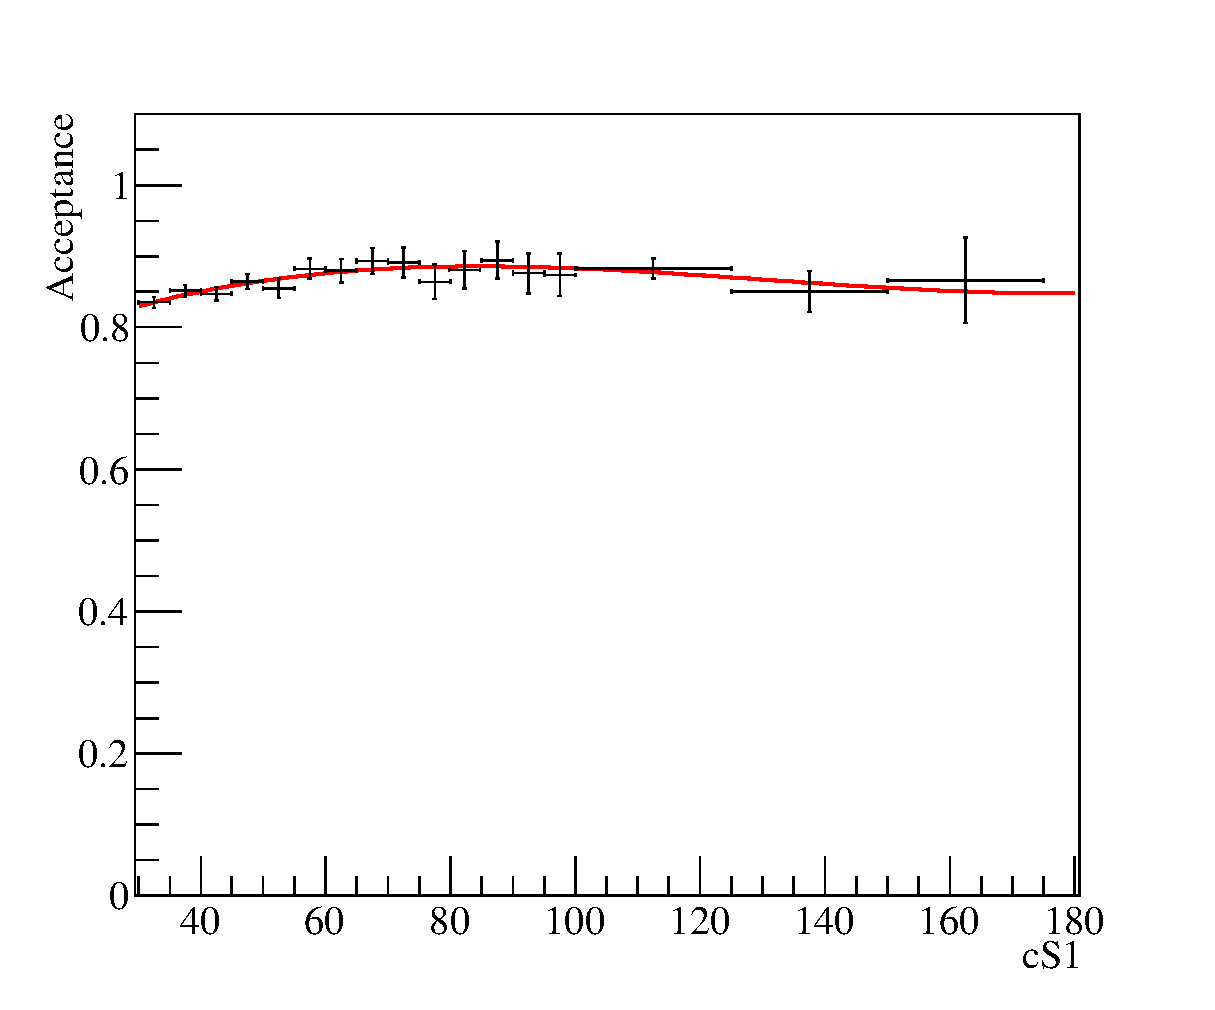
\includegraphics[width=1.\linewidth]{Figures/Acceptance.eps}}
\end{minipage}
\caption{The total acceptance of all cuts used, data from calibration in black and the fit in red.}
\label{fig:Acc}
\end{figure}

We define our signal region in the discrimination space (log(S2/S1) Vs S1). The upper bound is defined by taking the NR calibration sample mean and scaling it up such that in 30PE it coincide with the ER mean. From below the signal is bounded by taking 3 sigma from the NR mean, this is done for preventing gamma-X events to penetrate the sample. 

We divide our signal region into two bands in log(S2/S1). The bands are constructed such that the NR data sample is equally distributed between them. Each band is divided into several bins. The definition and content of each bin is presented in table~\ref{table:BinDef} and in Figure~\ref{fig:phasespace}. The main source of background is coming from ER leakage and hence, we estimate our background using calibration sample namely $^{232}Th$ and $^{60}Co$ to define the distribution between the bins. For sensitivity estimation we calculate a normalization factor in a sideband. For the final overall normalization we let the scaling factor be a free parameter to best fit the data.






\begin{table}
\resizebox{\columnwidth}{!}{

	 \begin{tabular}{|c| c| c| c| c| c |} 
 \hline
 Bin Number & Band Number & Lower E Limit & Higher E Limit & Number of Estimated Background Events & Number of Data Events \\  
 \hline\hline
 1 & 1 & 30  & 40  & 23.5 & 20 \\ 
 \hline
 2 & 1 & 40  & 50  & 15.7 & 17 \\
 \hline
 3 & 1 & 50  & 80  & 12.4 & 11 \\
 \hline
 4 & 1 & 80  & 120 & 1.1  & 1  \\
 \hline
 5 & 1 & 120 & 150 & 0.1  & 1  \\  
 \hline
 6 & 1 & 150 & 180 & 0.08 & 0  \\  
 \hline
 7 & 2 & 30  & 50  & 0.9  & 0  \\  
 \hline
 8 & 2 & 50  & 120 & 0.35 & 0  \\  
 \hline
 9 & 2 & 120 & 180 & 0.18 & 0  \\  
 \hline
\end{tabular}
}

\caption{Bins definition. The estimated background event is calculated by taking the calibration sample and scaling it by $6.54e-3$, which is a the ration between data and calibration in a sideband. The number of data events is the number of events from the DM data set in each bin.} \label{table:BinDef}

\end{table}


\begin{figure}[h!]
\begin{minipage}{1.\linewidth}
\centerline{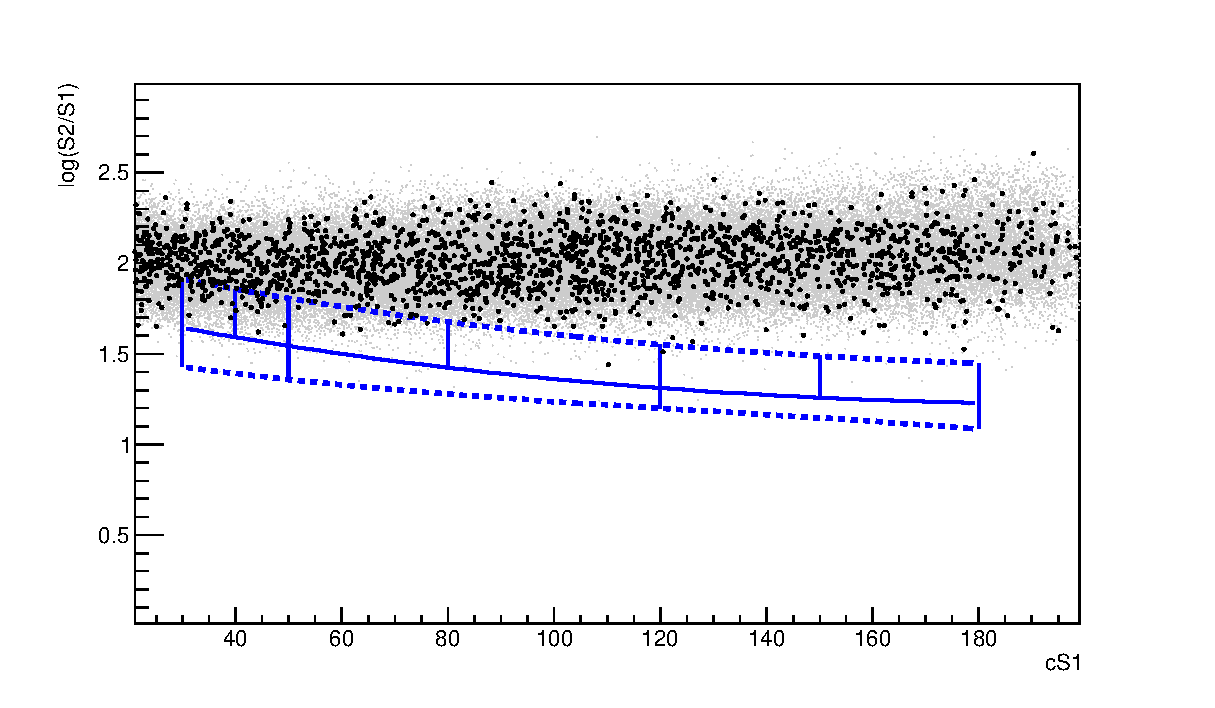
\includegraphics[width=1.\linewidth]{Figures/phasespace.eps}}
\end{minipage}
\caption{$^{Co}60$ and $^{232}Th$ data in light gray and DM data in black dots. The upper and lower limits of the energy region are in dotted blue, and the median and bins are in solid.}
\label{fig:phasespace}
\end{figure}  


\subsubsection{Low Energy}
\label{subsubsec:LowE}
short explanation on the bands on the background  uncertainties ref to run combination paper.


\subsection{Signal Model}
\label{subsec:SignalModel}
In order to estimate the energy deposition in the high E region we use the \Leff\ based method which is given in Eq.~\ref{eq:LeffEnergyScale}
\begin{equation}
\label{eq:LeffEnergyScale}
	E_{nr} = \frac{cS1}{L_y} \frac{1}{L_{eff}(E_{nr})} \frac{S_{ee}}{S_{nr}}
\end{equation}
The energy range in this region is bounded by the statistics of NR calibration data, namely $^{241}AmBe$.

The signal model is then produced by taking the event rate spectra converting it to S1, applying the acceptance and the detector response (explained in ~\cite{xe100_ana2012}) to give the expected event rate in the detector for each operator see Figure~\ref{fig:HighE}.
\begin{figure}[h!]
\begin{minipage}{1.\linewidth}
\centerline{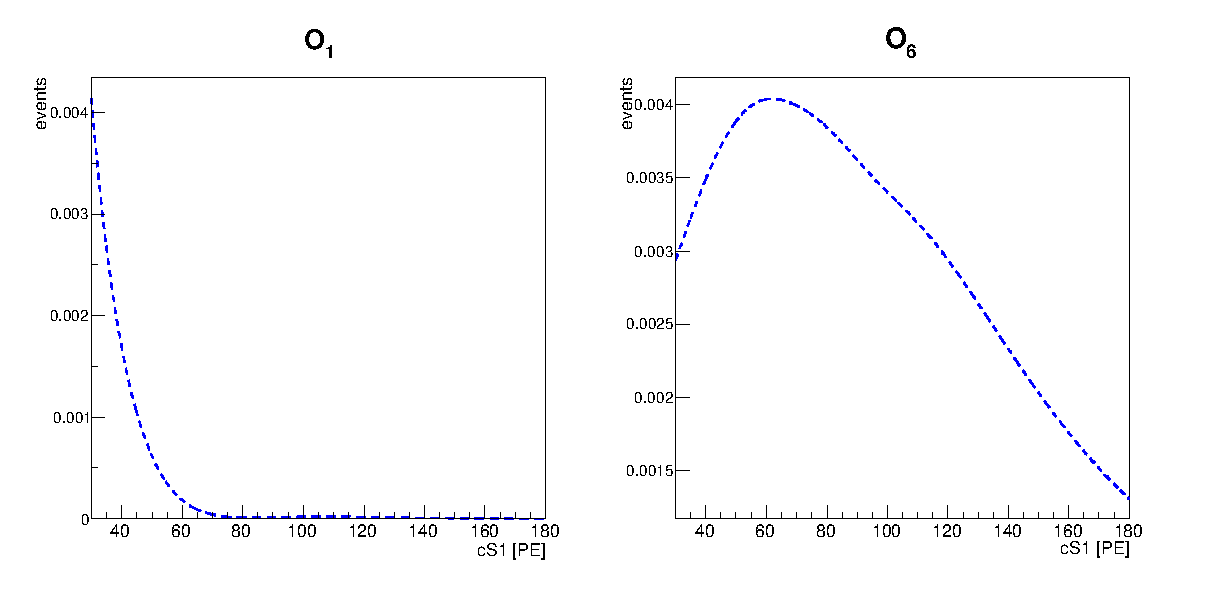
\includegraphics[width=1.\linewidth]{Figures/SigHighO1O6.eps}}
\end{minipage}
\caption{The expected signal in the high energy region for a 300 GeV/$c^2$ WIMP mass, Normalized to 5 events. Left(right) is the spectra for $O_1$($O_6$). Notice that for $O_1$ most of the events are not expected to deposit energy higher then 30 PE whereas for $O_6$ a large fraction of the events appear in this region.}
\label{fig:HighE}
\end{figure} 




\textbf{Ben add here} For the low energy region ...explain shortly the 2D signal model, and give ref to run combination paper. In fig~\ref{fig:LowE} is an example of the expected signal for $O_1$ and $O_6$ normalized to give 5 events in the total energy range (low E and high E)
\begin{figure}[h!]
\begin{minipage}{1.\linewidth}
\centerline{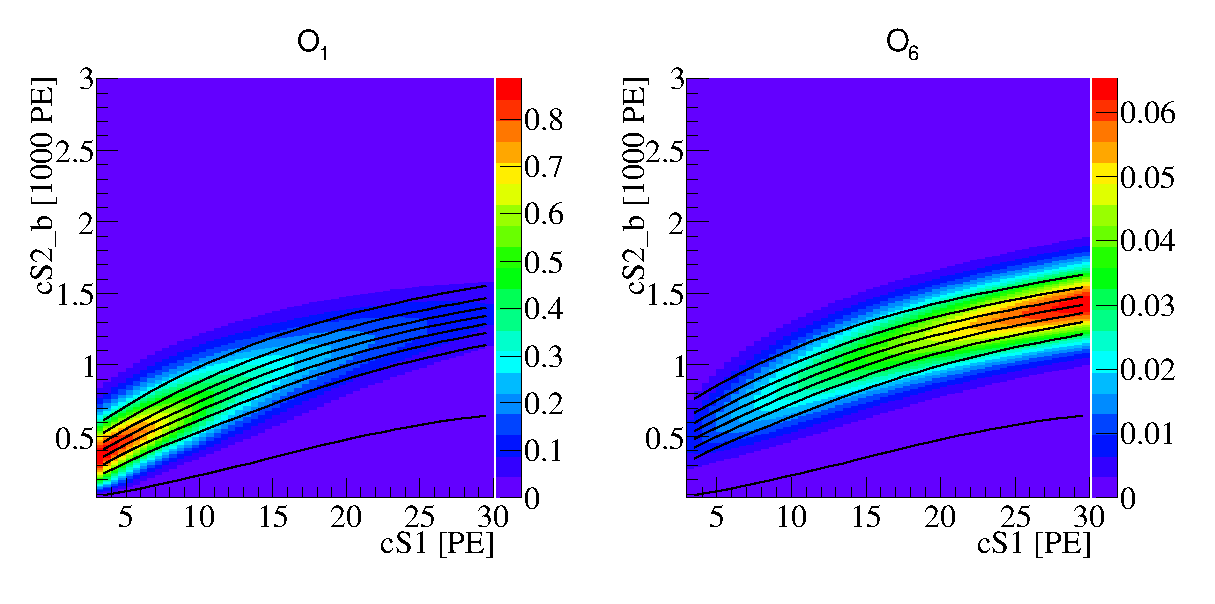
\includegraphics[width=1.\linewidth]{Figures/SigLowO1O6.eps}}
\end{minipage}
\caption{The expected signal in the low energy region for a 300 GeV/$c^2$ WIMP mass, Normalized to 5 events. Left(right) is the spectra for $O_1$($O_6$). Notice that for $O_1$ most of the events are expected to deposit energy lower then 30 PE whereas for $O_6$ a large fraction of the events do not appear in this region at all.}
\label{fig:LowE}
\end{figure}





\subsubsection{Elastic Scattering}
\label{subsubsec:Elastic}
Explain here how to get drde etc. give ref to fitzpatrick
\subsubsection{Inelastic Scattering}
\label{subsubsec:Inelastic}
explain the obtaining of inelastic and give ref to chang